\begin{usecase}{Extract Events from WhatsApp}
  \ucbasicinfo{High}{Regular}
  \ucshortdescription{System monitors WhatsApp messages of connected WhatsApp accounts and extract event details adding them to the user's calendar.}
  \uctrigger{A messages is sent to the connected WhatsApp account of an arbitrary user in our system.}
  \ucactors{WhatsApp}{}
  \ucpreconditions{At least one WhatsApp account must be connected.}
  \ucrelationships{Suggest Conflict Resolution}{N/A}{N/A}
  \ucinputsoutputs{
    \begin{itemize}
      \item \textbf{Messages sent to currently selected user} (Source: WhatsApp)
    \end{itemize}
  }{
    \begin{itemize}
      \item \textbf{Extracted event details} (Destination: System)
    \end{itemize}
  }
  \ucmainflow{
    \begin{enumerate}
      \item A sent message is received and the user has replied and 30 seconds have passed without any interruptions.
        \ucinfo{System reads a few messages before the current one to have context.}
      \item Add the detected event to the user's calendar.
        \ucinfo{Send a notification to the user telling them about the newly added event.}
    \end{enumerate}
  }
  \ucalternateflows{
    \begin{itemize}
      \item If there is a conflict adding this event, send a notification telling the user that there is a conflict they need to resolve.
    \end{itemize}
  }
  \ucexceptions{
    \begin{itemize}
      \item If there is an error during extraction of events, fail silently and log it to a specific table in the database for debugging later by developers.
    \end{itemize}
  }
  \ucconclusion{System successfully adds the event to the user's calendar and notifies the user of the added event.}
  \ucpostconditions{The event is added to the user's calendar.}
  \ucbusinessrules{
    \begin{itemize}
      \item Only messages with events and its surrounding context shall be analyzed.
      \item System must wait for user's reply before analyzing the messages.
      \item System must wait for 30 seconds before initiating the analysis on messages after the user replies and reset as long the conversation is onggoing.
    \end{itemize}
  }
  \ucspecialrequirements{The system must have access to the user's WhatsApp account as a client to receive and read messages.}
\end{usecase}

\begin{figure}[!h]
  \centering
  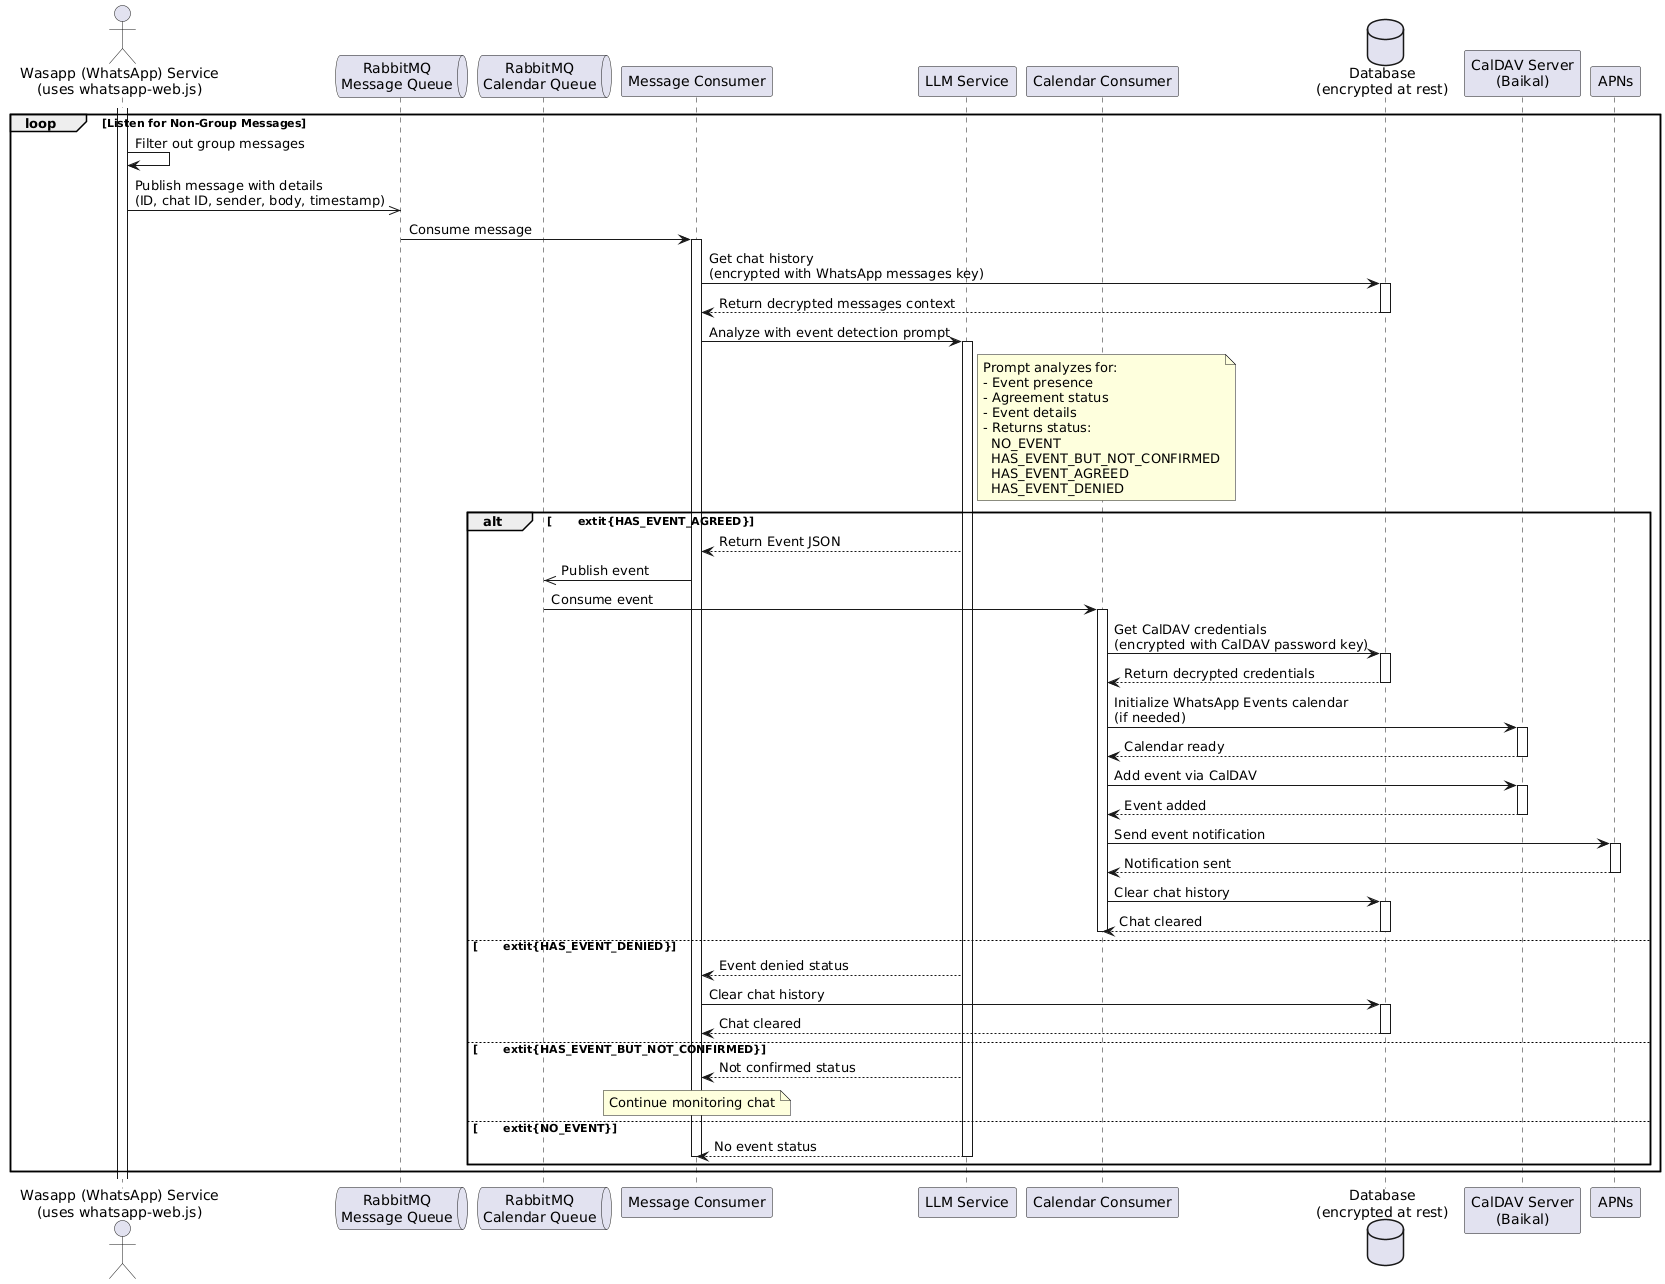
\includegraphics[width=\textwidth]{images/docs/diagrams/sequence-diagrams/all-sequence-diagrams/Extract Events from WhatsApp.png}
  \caption{Extract Events from WhatsApp Sequence Diagram}
  \label{fig:seq/extract-events-whatsapp}
\end{figure}